\subsection{Fault Modelling}
We focus on three faults: program counter fault, data fault and static instruction fault where program counter and data fault are considered transient, and static instruction fault is considered persistent, as described in \cref{sec:faultsce}.

\subsubsection{Program Counter Fault}
To model a single bit flip occurring in the program's execution, a special fault template is introduced, illustrated in \cref{fig:faultTime}. The template selects a random value between $0$ and the maximum possible global clock value, which represents when in the program's execution a fault happens. The random value is assigned to a global variable in the UPPAAL system.\\\\
Every instruction in the Java bytecode is represented by a location, and has an associated program counter. There are edges from each location going to the locations which can be reached if one bit is flipped in the program counter. These edges have guards which check whether the time the fault is injected, corresponds to the global clock at the time the model simulation is at that particular edge. If it is, the guard will allow the edge to be traversed. There are no fault edges going back to the added locations described in \cref{subsubsec:method}, since these are not a part of the original program and therefore do not have an associated program counter.
\begin{figure}[H]
\centering
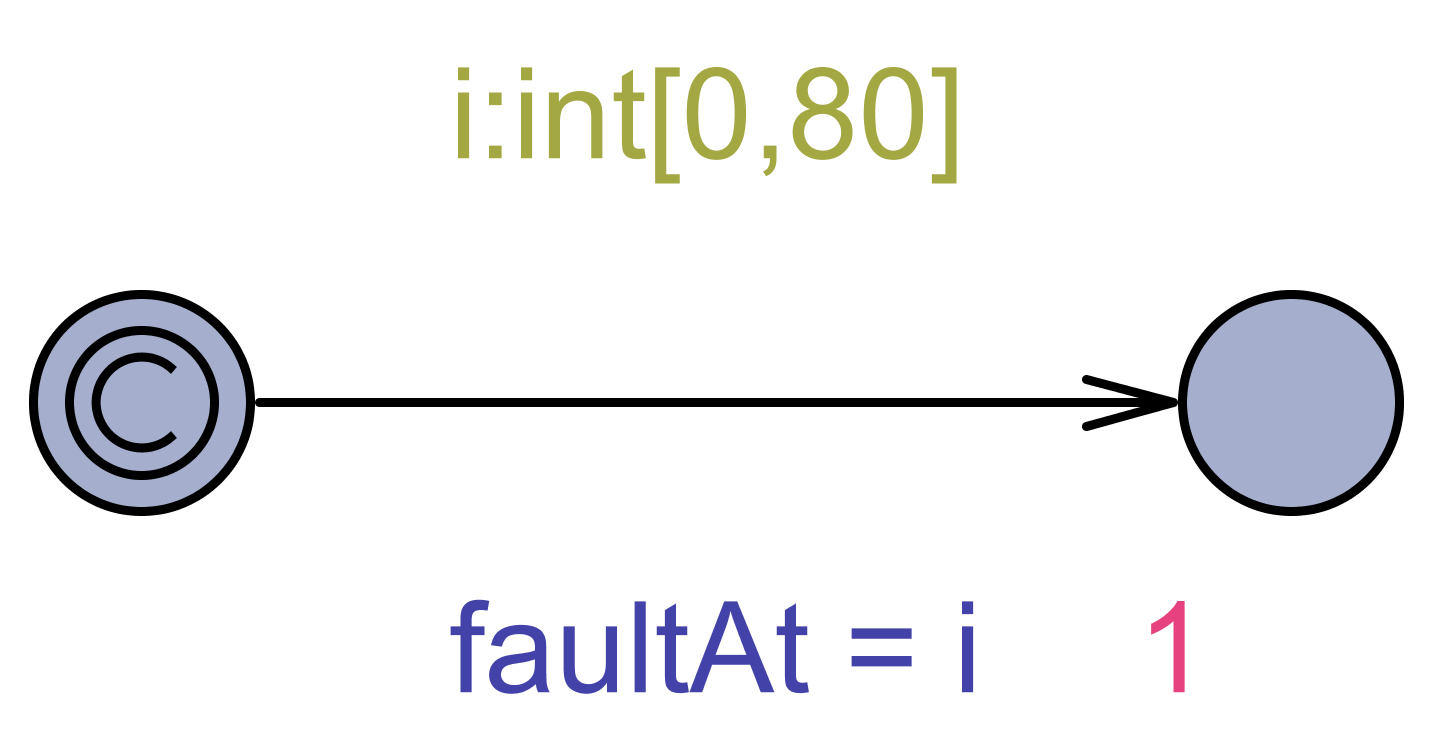
\includegraphics[width=0.3\textwidth]{figures/faulttemp.PNG}
\caption{The UPPAAL template which selects when to perform a bit flip in the program counter}
\label{fig:faultTime}
\end{figure}

\subsubsection{Data Faults}
% locals and opstack
To model a data fault being injected into the operand stack, a special template selects when a fault should be injected into the operand stack. 
This happens in the same way as in the program counter fault described earlier, illustrated in \cref{fig:faultTime}. 
The selected value is between $0$ and the maximum possible runtime of the program.
\cref{fig:opstackFlip} shows a method \texttt{getTriesRemaining}, in which a bit flip in the operand stack occurs.
Edges going back to the locations \texttt{pc0\_iconst\_2} and \texttt{pc0\_iconst\_2} are where the faults are introduced. These are added by the solution and are not a part of an unaltered model of a program. 
The edges have a guard, $faultTime \leq globalClock$, determined by the special template, which only allows a fault to happen if the program execution has executed for a certain amount of time. 
The fault itself is introduced by the update $os\lbrack osPos \rbrack\:\hat{}= 1 \ll osBitPos$, which flips bit \UPP{osBitPos} of value at position \UPP{osPos} in the operand stack.
\UPP{osBitPos} is a random value between $0$ and $7$, which denotes which bit should be flipp
ed. \UPP{osPos} is a random value between $0$ and the maximum size of the operand stack. 
After a fault has been introduced, the variable \UPP{faultTime} is set to a value higher than the maximum value of the global clock, to ensure only one fault happens per simulation.\\\\
Our approaches to modelling faults in the operand stack, heap and local variables are similar and therefore only one of them is described.
% 	% % % %
\begin{figure}[H]
\centering
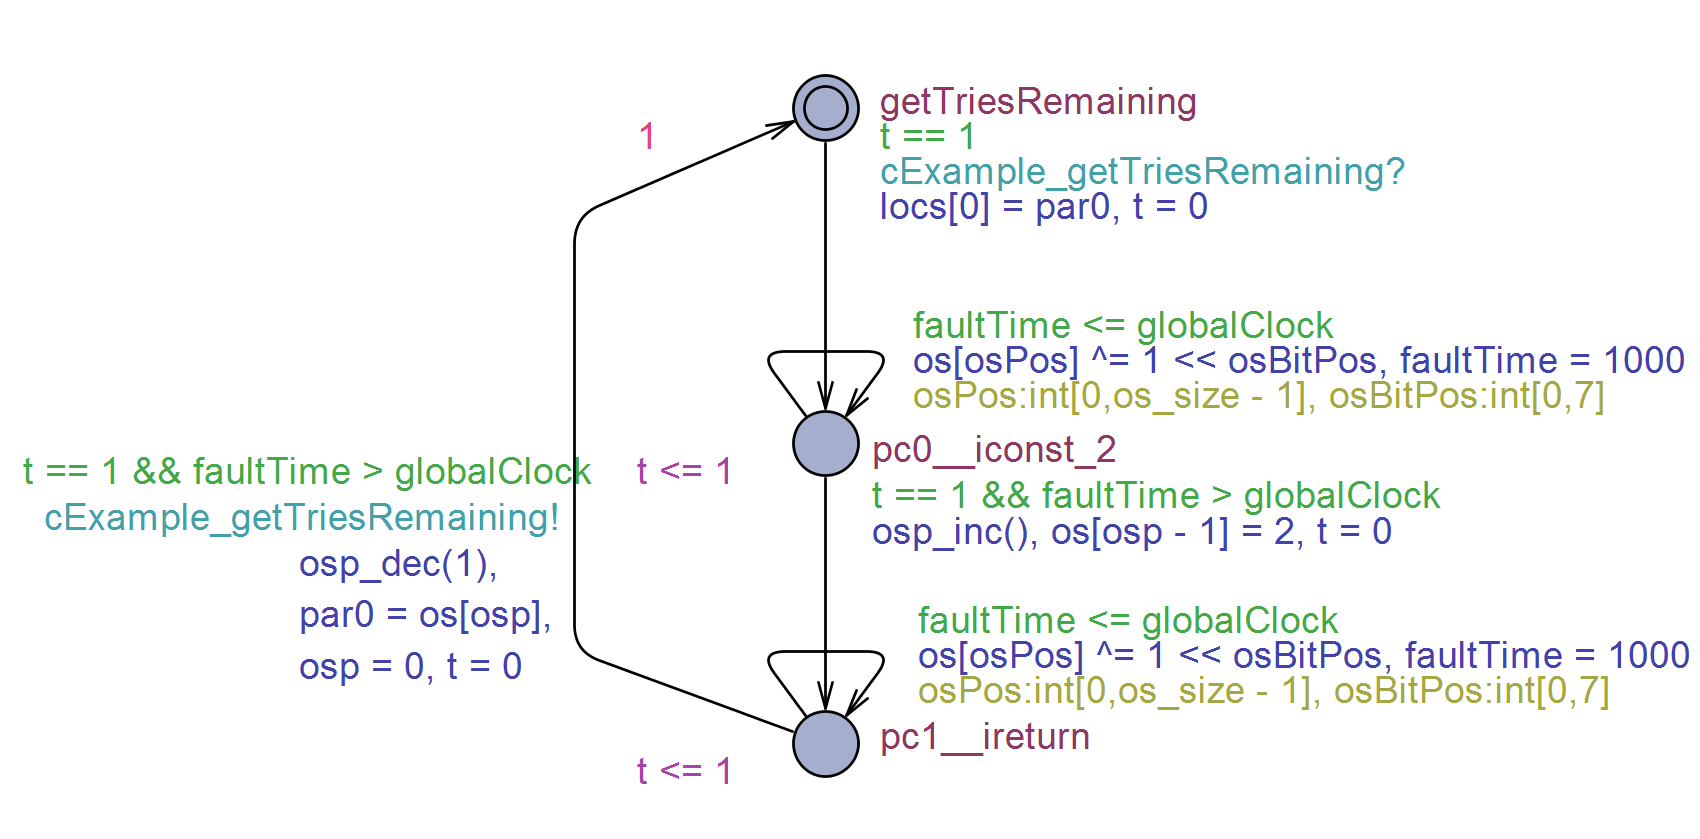
\includegraphics[width=\textwidth]{getTriesRemainnig.PNG}
\caption{The UPPAAL model af a method where a bit flip occurs in the operand stack.}
\label{fig:opstackFlip}
\end{figure}
\subsubsection{Instruction Fault}
An instruction fault is not necessarily time-dependent, i.e. it does not rely on a clock as the \textit{operand stack} fault described earlier. This fault model can represent both persistent and transient bit flips. The timing aspect of transient faults are modelled similar to operand stack faults, but persistent instruction faults are modelled by first assigning each edge of all templates a unique identifier. A special template then selects a random value in the range of $0$ and the greatest identifier in the modelled program. A fault will only happen once since only one identifier is selected, and only when the simulation reaches the instruction chosen by the fault template. This is enforced using guards which compares the selected identifier with the current edge's. During the generation of the model, the solution has calculated all instructions, an instruction can be changed to by a bit flip in their binary encoding. Additional edges are then inserted to perform the actions of the altered instructions. For example, the \texttt{ifeq} instruction, which can be bit flipped to \texttt{goto}, would cause an extra edge representing the "yes" branch to be created to the destination location of the original "yes" branch. The new edge is different from the two original edges by always being enabled, thus causing a simulation to always perform a jump regardless of the result of the \texttt{ifeq} comparison.